% Exposé III (continued): Theorem III.9 to Corollary III.13.
% Sources: theory/framework.md (Thm III.9 -- Cor III.13) and site/sections/06-fibres.html
% (#fibres-crossover to the end of the exposé). Proofs are in Appendix C.

\subsubsection{Two regimes and a crossover}\label{sec:fibres-crossover}

When the charge is a multiple of the identity, the LoRA flow has a closed form. Below a scale $\sigma^*$, one factor
carries the motion, as in LoRA-FA \citep{zhang2023lora}; above it, the factors share the work, as in balanced deep
linear networks.

\begin{theorem}{III.9}{closed-form isotropic-charge LoRA dynamics; known, \citet{xtarmoun2021understanding} and \citet{xmin2021explicit}}
Let $\rho(B,A)=W_{\mathrm{res}}+sBA$ be trained by gradient flow with rates $\eta_A,\eta_B$, and suppose the charge is
isotropic, $\Phi=-\kappa I_r$. Put $\mu=s\sqrt{\eta_A\eta_B}$ (a rate, unrelated to the moment map $\mu$ of
\thmref{Proposition}{III.7}), and on the locus where $Z=W-W_{\mathrm{res}}$ has rank $r$ write its compact SVD
$Z=U\Sigma V^\top$. Then
\[\dot W=-\mu^2\big[G\,V g_\kappa(\Sigma^2/\mu^2)V^\top+U f_\kappa(\Sigma^2/\mu^2)U^\top G\big],\]
where
\[f_\kappa(x)=\sqrt{x+\kappa^2/4}-\kappa/2,\qquad g_\kappa=f_\kappa+\kappa .\]
The identity holds pointwise on $\{\Phi=-\kappa I,\ \rk Z=r\}$; gradient flow is used only to keep $\Phi$ fixed. The
two terms under the root are equal at the \emph{crossover scale}
\[\sigma^*=\mu\lvert\kappa\rvert/2.\]
\begin{itemize}
\item For $\sigma\ll\sigma^*$ with $\kappa>0$, $f\to0$ and $g\to\kappa$, so $\dot W\approx-\mu^2\kappa\,GP_V$. These
  are LoRA-FA dynamics. The contribution of $A$ to $\dot W$ is $O(\sigma^2/(\mu^2\kappa))$, although $A$ itself still
  drifts slowly. For $\kappa<0$ the roles swap, $\dot W\approx-\mu^2\lvert\kappa\rvert P_UG$, and only $A$ effectively
  moves (Init[B]).
\item For $\sigma\gg\sigma^*$, $f\approx g\approx\sigma/\mu$, so
  \[\dot W\approx-\mu\big[G(Z^\top Z)^{1/2}+(ZZ^\top)^{1/2}G\big].\]
  These are the balanced dynamics of Arora, Cohen and Hazan.
\item \emph{Off the rank-$r$ locus.} Write $\dot W=-\mu^2(GS+TG)$ with $S=A^\top A/\eta_A$ and $T=BB^\top/\eta_B$, so
  that on the rank-$r$ locus $S=Vg_\kappa(\Sigma^2/\mu^2)V^\top$ and $T=Uf_\kappa(\Sigma^2/\mu^2)U^\top$. For
  $\kappa\ge0$, $T=f_\kappa(ZZ^\top/\mu^2)$ still holds as a full matrix function, but $S$ gains the term
  $\kappa(P_{\operatorname{row}A}-P_V)$; symmetrically, for $\kappa<0$, $T$ gains
  $\lvert\kappa\rvert(P_{\operatorname{col}B}-P_U)$. At the default-LoRA start $Z=0$ ($B_0=0$) this leaves
  $S=\kappa P_{\operatorname{row}A_0}$ and $T=0$, so $\dot W=-\mu^2\kappa\,GP_{\operatorname{row}A_0}$, and the
  $\sigma\ll\sigma^*$ regime extends continuously to $t=0$.
\end{itemize}
\end{theorem}

The closed form is due to \citet{xtarmoun2021understanding}, who call this charge ``$\lambda$-balanced'', and to
\citet{xmin2021explicit}; see also \citet{xdomine2025lazy} and \citet{xkunin2024get}. The balanced regime is that of
\citet{arora2018optimization}. The PEFT reading is ours. Panel (b) of Figure~\ref{fig:noether} shows the closed-form
singular-value dynamics and the crossover scale $\sigma^*$.

\noindent\labelsf{Num}\enspace The formula matches direct integration to $10^{-12}$, and the pointwise identity holds to
$10^{-15}$ for $\kappa\in\{-2,-0.3,0,0.3,2,10\}$ and all shape cases (Appendix~\ref{app:repro}).

\begin{explains}
Call this the PEFT reading; it is scoped to gradient flow and SGD.
\begin{itemize}
\item \emph{Default LoRA.} With $B_0=0$ and $A_0A_0^\top=cI$, $\kappa=c/\eta_A$ and
  $\sigma^*=\tfrac{sc}{2}\sqrt{\eta_B/\eta_A}$; HF's default gives $c\approx1/3$.
\item \emph{LoRA+} ($\lambda=\eta_B/\eta_A$) multiplies $\sigma^*$ by $\sqrt\lambda$ at fixed $\eta_A$, and its
  balanced-regime rate is the geometric mean $s\sqrt{\eta_A\eta_B}$. LoRA-FA is the endpoint $\lambda\to\infty$ of the
  LoRA+ family.
\item \emph{PiSSA at equal rates} has $\kappa=0$ and is exactly balanced forever under gradient flow; SGD drifts by
  $O(\eta^2)$ per step, and Adam does not preserve it.
\item \emph{Exactness.} The theorem is exact for EVA- and LoRA-GA-type orthonormal frames. For Kaiming initialisations
  it holds only approximately. The eigenvalues of $A_0A_0^\top$ lie near $c(1\pm\sqrt{r/n})^2$
  (\citealp{xmarchenko1967distribution}; \auxref{B.35}), so the crossover is a band of relative width $O(\sqrt{r/n})$ rather than a single
  scale. At $r=256$, $n=4096$, the eigenvalues of $3A_0A_0^\top$ span roughly $0.57$ to $1.57$.
\item \emph{Random $A$.} The one-sided regime fits the finding of \citet{zhu2024asymmetry} that a random, untrained $A$
  does nearly as well as a tuned one; the theorem says that this regime lasts while $\Delta W$ stays well below
  $\sigma^*$.
\end{itemize}
\end{explains}

\noindent\labelsf{Prediction}\enspace Under SGD, singular values of $\Delta W$ switch from one-sided to two-sided growth as they cross
$\sigma^*$ (\thmref{Prediction}{X.7}).

\subsubsection{The hyperparameter torus}\label{sec:fibres-torus}

Rescale block $i$ by $c_i$ and divide $s$ by the matching power of the $c_i$. The method is the same object of $\Meth$,
and training is the same if every step rescales alike. Adam ignores the size of a block's gradient, so its rate must
scale like $c_i$. An SGD step scales with the gradient, which shrinks by $c_i$, so its rate must scale like $c_i^2$.

\begin{theorem}{III.10}{the hyperparameter torus; the LoRA/Adam case is known, \citet{schulman2025lora}}
Let $\rho(q)=\theta_b+s\,\delta(q_1,\dots,q_k)$ with $\delta$ multihomogeneous of multidegree $(d_1,\dots,d_k)$. Train
block $i$ from $q_i(0)=\sigma_iu_i$ with Adam \citep{xkingma2015adam} ($\beta_1\in[0,1)$, $\beta_2\in(0,1)$, bias
correction allowed) at learning rate $\eta_i(t)$, on the loss $L\circ\rho$ with no $q$-dependent regulariser. Assume no
gradient clipping (or per-block clipping with thresholds rescaled as below), common random numbers (the same data order
and dropout masks in both runs), and exact arithmetic (the result is bit-exact in floating point when every $c_i$ is a
power of $2$). Then the trajectory $t\mapsto\rho(q(t))$ is invariant under the torus action of $c\in\R_{>0}^k$:
\[\big(s,\ \eta_i(t),\ \sigma_i,\ \varepsilon_i,\ \lambda_i,\ C_i\big)\mapsto\Big(s\prod_ic_i^{-d_i},\ c_i\eta_i(t),\ c_i\sigma_i,\ \varepsilon_i/c_i,\ \lambda_i/c_i,\ C_i/c_i\Big).\]
Here $\varepsilon_i$ is a per-block Adam $\varepsilon$ (with the convention $0/0=0$ at $\varepsilon=0$), $\lambda_i$ a
per-block decoupled (AdamW) weight decay, and $C_i$ a per-block clipping threshold. Under SGD, with or without
heavy-ball or Nesterov momentum, the same holds with $\eta_i(t)\mapsto c_i^2\eta_i(t)$ and coupled $L^2$ decay
$\lambda_i\mapsto\lambda_i/c_i^2$. In particular, any learning-rate schedule shared by all blocks, warm-up included, is
preserved.
\end{theorem}

The LoRA/Adam case, with the $\varepsilon>0$ extension and the two effective hyperparameters, is due to
\citet{schulman2025lora} (\emph{LoRA Without Regret}). New here are arbitrary multihomogeneous $\delta$ and the SGD and
heavy-ball $c^2$ law.

\noindent\labelsf{Num}\enspace Trajectory differences are exactly $0.0$ for power-of-two $c$ and about $10^{-15}$ otherwise,
including a warm-up schedule and rescaled $\varepsilon$ and decay. With $\varepsilon$ or decay held fixed, or with
global-norm clipping, they are $10^{-3}$ to $O(1)$ (Appendix~\ref{app:repro}).

\begin{explains}
Only the torus orbit of the hyperparameters reaches the weights. LoRA is the case $k=2$, $d=(1,1)$; $\delta$ may be any
multilinear update, such as that of VeRA \citep{kopiczko2023vera} in its two scaling vectors or that of LoHa
\citep{hyeonwoo2021fedpara} in its four factors.
\end{explains}

\begin{corollary}{III.11}{LoRA+ is $\alpha$ in disguise; rsLoRA is LoRA; (a) and the LoRA+ reading are known, \citet{schulman2025lora}}
For linear LoRA modules ($k=2$, $d=(1,1)$, $\sigma_B=0$), under the hypotheses of \thmref{Theorem}{III.10}:

(a) \emph{Effective hyperparameters.} Under Adam the torus invariants of $(s,\eta_A,\eta_B,\sigma_A)$ are
$(s\eta_A\eta_B,\ \sigma_A/\eta_A)$; the quantities $\alpha\cdot\mathrm{init}_A\cdot\mathrm{LR}_B$ and
$\mathrm{init}_A/\mathrm{LR}_A$ of Schulman et al.\ are equivalent generators. Under SGD the invariants are
$(s^2\eta_A\eta_B,\ \sigma_A^2/\eta_A)$.

(b) \emph{LoRA+.} Under Adam with $\varepsilon=0$, no weight decay, no gradient clipping and a learning-rate schedule
shared by both groups, LoRA+ with ratio $\lambda$ at scale $s$ produces \emph{exactly} the trajectory of plain LoRA at
scale $\lambda s$ (same $\eta_A$, same $A_0$). For $\varepsilon>0$ the equivalence needs a per-block
$\varepsilon_B'=\lambda\varepsilon$, and with AdamW a per-group decay $\lambda\cdot\mathrm{wd}$ on $B$. Under SGD it
holds at scale $\sqrt\lambda\,s$, or equivalently with plain LoRA at the single rate $\sqrt{\eta_A\eta_B}$ and
$A_0\mapsto\lambda^{1/4}A_0$.

(c) \emph{rsLoRA.} $\rho_{\mathrm{rs}}(B,A)=\rho_{\mathrm{LoRA}}(\sqrt r\,B,A)$ is an isomorphism of objects. Up to the
hyperparameter torus, rsLoRA can be represented as LoRA at the same $\alpha$ with $\eta_B$ multiplied by $\sqrt r$ under
Adam (by $r$ under SGD), or equally as LoRA with $\alpha$ multiplied by $\sqrt r$ at the same rates. The reading ``same
object, different metric'' is a choice of representative within the orbit. Part (c) concerns a fixed rank; it does not
address rsLoRA's rank-stability prescription, how $\alpha$ should scale with $r$.
\end{corollary}

LoRA+ is due to \citet{hayou2024lora}, rsLoRA to \citet{kalajdzievski2023rank}, and (a) with the LoRA+ reading to
\citet{schulman2025lora}. On the empirical side, \citet{lee2026learning} find that nine LoRA variants reach similar peak
performance once the learning rate is tuned.

\noindent\labelsf{Num}\enspace The maximum trajectory difference is exactly $0.0$ at $\varepsilon=0$ for power-of-two
$\lambda$ and about $10^{-14}$ otherwise, against $0.93$ for the unrescaled control. It is $5\times10^{-9}$ at a shared
$\varepsilon=10^{-8}$, and $0.6$ with global-norm clipping at $0.5$ (Appendix~\ref{app:repro}).

\begin{explains}
LoRA's four knobs are coordinates on a 4-dimensional space acted on by a 2-torus, and only the orbit matters. LoRA+,
rsLoRA and $\alpha$-tuning therefore collapse into one family. The slogan depends on the chart. Holding $\eta_A$ fixed,
LoRA+ is ``$\alpha$ multiplied by $\lambda$''; holding $\eta_B$ fixed, it is plain LoRA with $\eta_A$ divided by
$\lambda$, a slower $A$-timescale. In particular, Adam does not make the LoRA+ ratio non-absorbable.
\end{explains}

\noindent\labelsf{Prediction}\enspace Any gain of LoRA+ over LoRA with $\alpha$ re-tuned by the factor $\lambda$ must come from the
ingredients that break the extended torus: global-norm clipping (on by default in the HF Trainer,
\texttt{max\_\allowbreak grad\_\allowbreak norm=1.0}), $\varepsilon$ or weight decay held equal across parameter groups (as in HF PEFT's LoRA+
optimizer), and learning-rate schedules that differ between groups. Shared schedules and warm-up preserve the torus.
HF's LoRA+ optimizer treats embedding adapters and 1-D parameters separately, so the statement covers linear modules
only (\thmref{Prediction}{X.1}).

\begin{figure}[tbp]
\centering
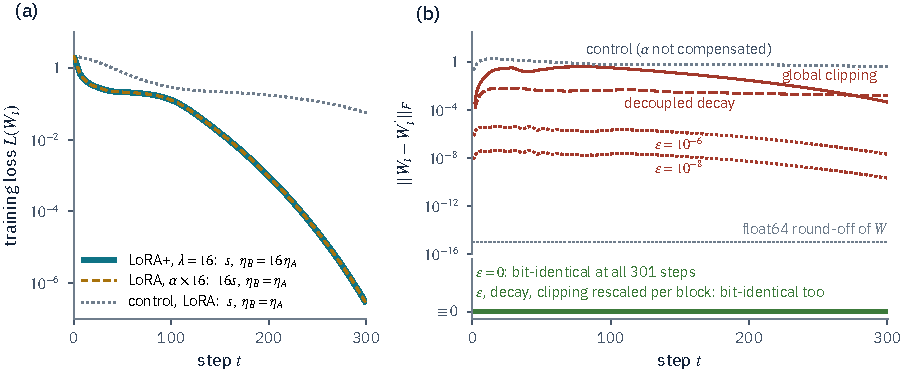
\includegraphics[width=\linewidth]{figures/orbit}
\caption{\textbf{LoRA+ is $\alpha$ in disguise} (\thmref{Theorem}{III.10}, \thmref{Corollary}{III.11}). A seeded toy LoRA regression with $B_0=0$ is trained by Adam in float64, once as LoRA+ with ratio $\lambda=16$ (scale $s$, $\eta_B=16\,\eta_A$) and once as plain LoRA with $\alpha$ multiplied by $16$ (scale $16s$, $\eta_B=\eta_A$), at the same $\eta_A$ and $A_0$. (a)~At $\varepsilon=0$, without weight decay or clipping, the two loss curves coincide; the control, plain LoRA at the uncompensated scale $s$, ends far above them. (b)~The weight gap $\lVert W_t-W'_t\rVert_F$ between the two runs at every step, on a log scale above an exact-zero floor. At $\varepsilon=0$ the runs are bit-identical at every step: the torus element relating them, $c=(1,1/16)$, is a power of two and rescales floating-point numbers exactly. Each red curve switches on one ingredient with a single value shared by both parameter groups: Adam's $\varepsilon$, decoupled weight decay, or global-norm clipping. Each breaks the hyperparameter torus; the control is dotted. Rescaling the same ingredients per block, as \thmref{Theorem}{III.10} prescribes, restores the exact zero (green floor). The values used are in \S\ref{app:repro-figures}.}
\label{fig:orbit}
\end{figure}

\subsubsection{What the optimizer can see}\label{sec:fibres-hierarchy}

An optimizer is equivariant under a gauge element $g$ if starting from $(Bg^{-1},gA)$ gives the transported trajectory.
The Euclidean metric of SGD respects rotations of the rank channels. Adam, acting coordinatewise, respects only the
signed permutations.

\begin{remark*}{2026: privacy noise}
Privacy noise fits the same pattern. DP-SGD \citep{xabadi2016deep} on the factors adds isotropic Gaussian noise $\xi$ to
the clipped factor gradients, and $\xi g^{-1}$ has the law of $\xi$ only for orthogonal $g$, so it respects $\Ort(r)$
and no larger subgroup. PRISM \citep{wang2026prism} clips and noises the projection of each gradient onto the tangent
space of $\MM_r$ at $BA$, which depends only on $\operatorname{col}B$ and $\operatorname{row}A$. For full-rank factors
the privatised gradient then has the same law for every factorisation of $BA$. Its Algorithm 1 then applies damped
$r\times r$ preconditioners (its Eqs.~24--26), which the paper also calls gauge invariant. They respect only $\Ort(r)$.
Under $(B,A)\mapsto(cB,A/c)$ the preconditioned factor steps do not change, so $\delta B\,A$ scales by $1/c$ and
$B\,\delta A$ by $c$. The released code returns to balanced factors, $B^\top B=AA^\top$, after every step, where the
remaining gauge is $\Ort(r)$.
\end{remark*}

\begin{theorem}{III.12}{the optimizer gauge hierarchy}
On LoRA's full-rank locus, with hyperparameters shared by all rank channels, the largest subgroup of the gauge $\GL_r$
under which an update rule is equivariant, at the level of parameters, is as follows.

(a) SGD and GD with any block rates, with or without heavy-ball momentum: $\Ort(r)$.

(b) Adam and AdamW at fixed learning rates ($\beta_1,\beta_2\in[0,1)$, any $\varepsilon\ge0$, any weight decay): the
signed permutations $B_r$, of order $2^rr!$. A positive diagonal $g=\diag(d)$ is a symmetry only \emph{jointly} with
per-rank-channel hyperparameters, and only without global-norm clipping. At $\varepsilon=0$ and without weight decay it
suffices to rescale the rates, $\eta_{B,j}\mapsto\eta_{B,j}/d_j$ and $\eta_{A,j}\mapsto d_j\eta_{A,j}$. With
$\varepsilon>0$ one must also give each channel its own $\varepsilon_{B,j}=d_j\varepsilon$ and
$\varepsilon_{A,j}=\varepsilon/d_j$. With decoupled decay multiplied by the learning rate (PyTorch AdamW) one must also
set $\lambda_{B,j}=d_j\lambda$ and $\lambda_{A,j}=\lambda/d_j$; under the convention of \citet{xloshchilov2019decoupled},
where decay is scaled only by the schedule multiplier, $\lambda$ needs no change.

(c) Undamped scaled GD ($\delta=0$; the Riemannian preconditioner of Tong, Ma and Chi and of Zhang and Pilanci, with or
without heavy-ball momentum): all of $\GL_r$. The $W$-trajectory from gauge-related initial states (with zero or
correspondingly transformed momentum) is independent of the representative; a step may drop rank, so the iteration maps
into $W_0+\Mr$.
\end{theorem}

Scaled GD is due to \citet{xtong2021accelerating} and \citet{zhang2024riemannian}. LoRA-RITE \citep{yen2024lora} makes
gauge invariance a design requirement for LoRA optimizers and reports that it pays.

\paragraph{Published variants} Damped scaled GD ($\delta>0$) is only $\Ort(r)$-equivariant. Wrapped in AdamW, as in
Zhang and Pilanci's scaled AdamW (their practical variant) and in HF's \texttt{create\_\allowbreak riemannian\_\allowbreak optimizer}, it is
$B_r$-equivariant by (b). The first-order $W$-level dynamics of LoRA-Pro \citep{wang2024lorac} descend
(\thmref{Proposition}{III.4}(b)), and so do those of its variant with free matrix $X=0$; its published parameter update
with the Sylvester-optimal $X$ is only $\Ort(r)$-equivariant, and its discrete $W$-step depends on the representative at
$O(\eta^2)$. LoRA-RITE states only $W$-level invariance (its Definition 1). Its update (unmagnified gradients,
transported matrix moments, then multiplication by $(R_B^\top)^+$) is $\GL_r$-equivariant at the parameter level on the
full-rank locus: under a gauge change its internal quantities change only by orthogonal matrices, and the final
multiplication supplies the gauge element (Appendix~\ref{proof:III.12}, which follows its Algorithm~1 line by line; the
resulting step is Eq.~15 of \citet{yen2024lora}). LoRA-RITE is therefore an Adam-type optimizer in class (c).

\noindent\labelsf{Num}\enspace For Adam, the defects are $10^{-15}$ for signed permutations, $11.3$ for a positive
diagonal, $6.6$ for a rotation, and $5\times10^{-16}$ for the diagonal with jointly rescaled per-channel rates at
$\varepsilon=0$. With $\varepsilon=10^{-8}$ left unrescaled the joint torus fails by about $2\%$. LoRA-RITE (its
Algorithm 1) from $(B,A)$ and from $(Bg^{-1},gA)$ with a generic $g$ agrees to $3\times10^{-14}$ over 30 steps
(referee replication). LoRA-Pro with the Sylvester $X$ has a parameter-level defect of $1.2$ under a non-orthogonal $g$,
against $2\times10^{-15}$ with $X=0$ or with an orthogonal $g$ (Appendix~\ref{app:repro}).

\begin{explains}
There is a hierarchy $B_r\subset\Ort(r)\subset\GL_r$ of optimizer geometries, strict for $r\ge2$. $\GL_r$-equivariant
rules, started from gauge-related states, define an optimizer on the \emph{model} rather than on a chart. More generally
any rule that maps gauge orbits to gauge orbits does (for instance a step followed by a canonical refactorisation of
$W$), while $B_r$- and $\Ort(r)$-equivariant rules in general do not. Plain Adam, the default, sees a finite shadow of
the gauge. LoRA+ and rsLoRA act on the hyperparameter torus (\thmref{Theorem}{III.10}) and leave the gauge of a fixed
method alone; balanced or orthonormal initialisations choose a point in the fibre. The positive torus is a symmetry of
the \emph{hyperparameters}; Adam at fixed rates does not have it.
\end{explains}

\begin{figure}[tbp]
\centering
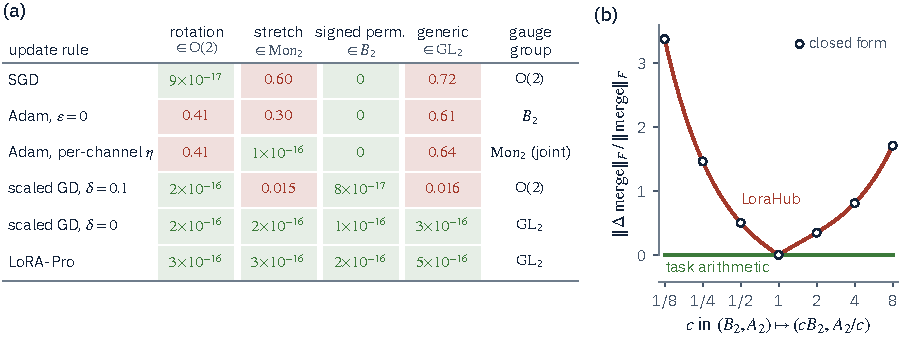
\includegraphics[width=\linewidth]{figures/gauge}
\caption{\textbf{Update rules that see the gauge} (\thmref{Theorem}{III.12}, \thmref{Proposition}{III.4}, \thmref{Proposition}{V.4}). (a)~At a fixed seeded LoRA state $(B,A)$ with loss gradient $G$, each cell is the relative gauge defect $\lVert\delta W(g)-\delta W(I)\rVert_F/\lVert\delta W(I)\rVert_F$ of one update rule: the change in its first-order weight update $\delta W=\delta B\,A+B\,\delta A$ when the factors are replaced by the gauge-equivalent pair $(Bg^{-1},gA)$. The columns are a rotation, a stretch, a signed permutation and a generic $g\in\GL_2$; under each name is the smallest of the groups $B_2=\Ort(2)\cap\mathrm{Mon}_2$, $\Ort(2)$, $\mathrm{Mon}_2$ (monomial matrices) and $\GL_2$ that contains it. Green cells vanish up to float64 round-off, and they occur exactly where $g$ lies in the rule's gauge group (right column): $\Ort(2)$ for SGD and for damped scaled GD, $B_2$ for Adam, $\mathrm{Mon}_2$ for Adam whose per-rank-channel rates are rescaled jointly with a stretch, and all of $\GL_2$ for undamped scaled GD and for LoRA-Pro with the Sylvester-optimal free matrix, whose weight updates depend only on $W$. Red cells are genuine defects. (b)~Three LoRA modules $(B_i,A_i)$ with weights $w_i$ are merged after module~2 alone is re-gauged to $(cB_2,A_2/c)$. Task arithmetic \citep{ilharco2022editing}, $\sum_iw_iB_iA_i$, does not move. The LoraHub merge \citep{huang2023lorahub}, $(\sum_iw_iB_i)(\sum_jw_jA_j)$, does, and the open circles, the closed form of \thmref{Proposition}{V.4}, match the recomputed change. The settings are in \S\ref{app:repro-figures}.}
\label{fig:gauge}
\end{figure}

\subsubsection{What a zero-\texorpdfstring{$B$}{B} start chooses}\label{sec:fibres-zero-b}

Default LoRA starts at $B_0=0$ with a random full-rank $A_0$. The image remembers only $\operatorname{row}A_0$
(\thmref{Theorem}{II.2}). Training remembers what the optimizer's gauge group cannot move.

\begin{corollary}{III.13}{what a zero-$B$ initialisation really chooses}
At $q_0=(0,A_0)$ with $\rk A_0=r$, with hyperparameters shared by the rank channels and the same data order and dropout
masks, two choices of $A_0$ give the same $\theta$-trajectory whenever the optimizer's gauge group relates them. The
resulting invariant of $A_0$ is:
\begin{itemize}
\item $\operatorname{row}A_0\in\Gr(r,n)$ for an update rule that is $\GL_r$-equivariant at every point of its
  trajectory, including $B=0$ and rank-deficient $B$, run without global-norm clipping. An example is
  $\delta B=-\eta\nabla_B(AA^\top)^{-1}$, $\delta A=-\eta(AA^\top)\nabla_A$, which needs only $\rk A=r$;
\item the PSD matrix $A_0^\top A_0$ for SGD, which is exactly the initial preconditioner in
  \[\dot W(0)=-s^2\eta_BGA_0^\top A_0;\]
\item $A_0$ up to signed permutation of its rows for Adam.
\end{itemize}
The undamped scaled-GD optimizers of \thmref{Theorem}{III.12}(c) are not defined at $B=0$, since they need
$(B^\top B)^{-1}$. LoRA-RITE uses pseudo-inverses and so is defined there, but its $\GL_r$-equivariance is established
only on the full-rank locus. Their damped forms are only $\Ort(r)$-equivariant, so in practice their invariant is a
$\delta$-dependent function of $A_0^\top A_0$, and their Adam-wrapped forms (Riemannian-preconditioned AdamW, HF's
LoRA-FA optimizer) have the invariant $A_0$ modulo $B_r$. Conversely, different invariants give different dynamics, for
SGD and for Adam at $\varepsilon=0$.

Random-$A$ LoRA and EVA are different points of the $B=0$ stratum $\{(0,A):\rk A=r\}$ of the apex fibre
$\rho^{-1}(\theta_0)=\{(B,A):BA=0\}$; Init[B] lies in another stratum of the same fibre. LoRA-FA is a different
\emph{object}, the sub-object $\mathrm{FA}(A_0)\hookrightarrow\mathrm{LoRA}_{(0,A_0)}$ (\thmref{Proposition}{I.8}). More
precisely, EVA is a point of the apex fibre of $\mathrm{LoRA}_{r_l}$ at its per-layer redistributed rank and adjusted
$\alpha$, with orthonormal rows only when \texttt{whiten=False}.
\end{corollary}

Appendix~\ref{proof:III.13} proves the converse (different invariants give different dynamics) by comparing first
steps. \citet{hayou2024impact} showed that the two zero-product starts, random $A$ with
$B=0$ and random $B$ with $A=0$, train differently; here they lie in different strata of one apex fibre, with charges of
opposite sign. EVA \citep{paischer2024parameter} and random-$A$ LoRA share a stratum.

\noindent\labelsf{Num}\enspace SGD from $A_0$ and from $QA_0$ (with $Q$ orthogonal) agree to $10^{-15}$, and from $A_0$
and $DA_0$ (with $D$ diagonal) differ by $0.81$. Adam from $A_0$ and from $PA_0$ (with $P$ a signed
permutation) agree to $10^{-16}$, and from $A_0$ and $QA_0$ differ by $0.98$. The example rule from $A_0$ and from
$gA_0$ agrees to $3\times10^{-15}$. LoRA-RITE's Algorithm 1, run as written with its pseudo-inverses from $B_0=0$, gives
the same weights from $A_0$ and from $gA_0$ for a generic $g$ to $10^{-13}$, and weights that differ by $O(1)$ for a
different row space (Appendix~\ref{app:repro}).

\begin{explains}
The strata of \thmref{Theorem}{II.2} are the expressive quotient. The dynamics see a finer quotient, and how fine depends
on the optimizer (Table~\ref{tab:zero-b}). Undamped scaled GD is undefined at $B=0$, so scaled-GD optimizers enter in
damped ($\Ort(r)$) or AdamW-wrapped ($B_r$) form.
\end{explains}

\begin{table}[t]
\centering
\caption{What an update rule reads off $A_0$ from a zero-$B$ start (\thmref{Corollary}{III.13}).}
\label{tab:zero-b}
\small
\begin{tabularx}{\linewidth}{>{\raggedright\arraybackslash}X l >{\raggedright\arraybackslash}p{4.6cm}}
\toprule
\headrow \textbf{Update rule} & \textbf{Equivariance group} & \textbf{What it reads off $A_0$ at $B_0=0$}\\
\midrule
$\GL_r$-equivariant along the whole trajectory (the example rule; LoRA-RITE's Algorithm 1, checked numerically) & $\GL_r$ & $\operatorname{row}A_0\in\Gr(r,n)$\\
SGD, GD & $\Ort(r)$ & $A_0^\top A_0$\\
damped scaled GD & $\Ort(r)$ & $A_0^\top A_0$ (through a $\delta$-dependent function)\\
Adam, AdamW; scaled AdamW (Zhang and Pilanci; HF's Riemannian optimizer with AdamW); HF's LoRA-FA optimizer & $B_r$ & $A_0$ up to signed permutation of its rows\\
\bottomrule
\end{tabularx}
\end{table}

Two problems stay open. One is the apex fibre modulo $B_r$ for Adam, stratified by $\Phi_0$, degenerate pointings
included. The other is an Adam analogue of \thmref{Theorem}{III.9}, a conserved or monotone quantity for sign-like
updates.

Exposé~\ref{sec:lens} reads the same cometric from the backward side of the lens, where methods that compress gradients
have cometrics of their own.
